\documentclass[10pt]{extarticle}
\usepackage[utf8]{inputenc}
\usepackage[T1]{fontenc}
\usepackage[brazil]{babel}
\usepackage[a4paper,margin=1.3cm]{geometry}
\usepackage{graphicx,booktabs,hyperref,setspace,enumitem}
\setlist{nosep,leftmargin=1.2em}
\setlength{\parindent}{0pt}
\setlength{\parskip}{2pt}
\setlength{\tabcolsep}{4pt}
\renewcommand{\arraystretch}{0.95}
\pagestyle{empty}
\begin{document}
\begin{center}
{\large\bfseries Classificação no dataset Iris: estatísticas, PCA e K-NN}\\[2pt]
Gustavo Jakobi GRR20221253 \quad Bruno Crestani GRR20221240\\[1pt]
Código: \url{https://github.com/GJakobi/iris-knn-pca}
\end{center}

\textbf{Dados.} UCI Iris: 150 amostras, 4 variáveis (cm) e 3 classes balanceadas (50 amostras cada).

\textbf{1. Estatísticas} (média / desvio / moda).
\begin{center}\footnotesize
\begin{tabular}{lcccc}
\toprule
 & Geral & Setosa & Versicolor & Virginica \\
\midrule
sepal\_length & 5,84/0,83/5,0 & 5,01/0,35/5,0 & 5,94/0,52/5,5 & 6,59/0,64/6,3 \\
sepal\_width  & 3,05/0,43/3,0 & 3,42/0,38/3,4 & 2,77/0,31/3,0 & 2,97/0,32/3,0 \\
petal\_length & 3,76/1,76/1,5 & 1,46/0,17/1,5 & 4,26/0,47/4,5 & 5,55/0,55/5,1 \\
petal\_width  & 1,20/0,76/0,2 & 0,24/0,11/0,2 & 1,33/0,20/1,3 & 2,03/0,28/1,8 \\
\bottomrule
\end{tabular}
\end{center}

\textbf{2. Comprimento $\times$ largura} (correlação de Pearson).
\begin{center}\footnotesize
\begin{tabular}{lccc}
\toprule
 & Setosa & Versicolor & Virginica \\
\midrule
Sépala & 0,75 & 0,53 & 0,46 \\
Pétala & 0,31 & 0,79 & 0,32 \\
\bottomrule
\end{tabular}
\end{center}
A sépala tem correlação positiva nas três classes. Na pétala, só a versicolor tem correlação forte.
A setosa forma um grupo separado nos dois gráficos.

\begin{center}
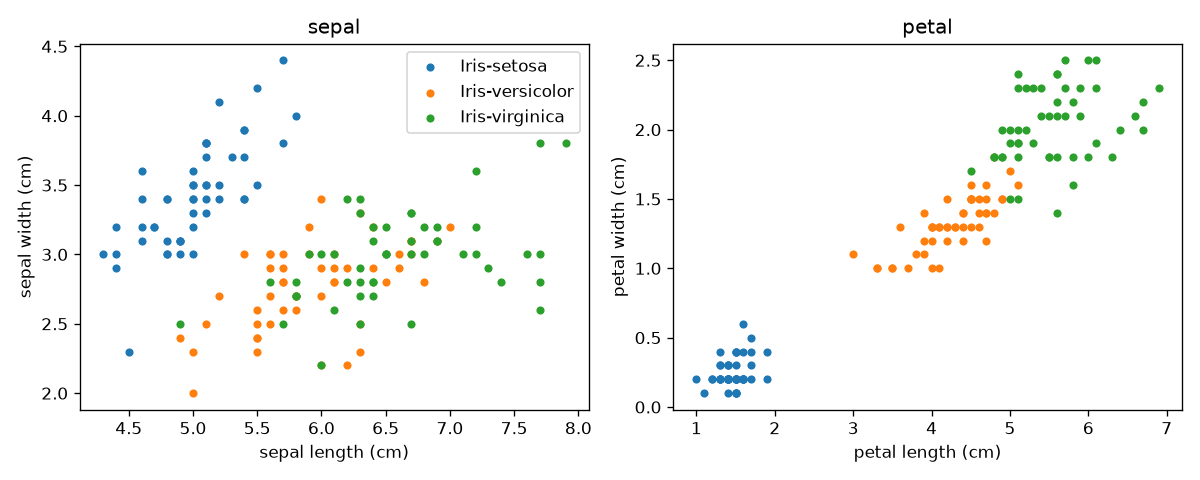
\includegraphics[height=4.2cm]{fig_relacao.png}\hfill
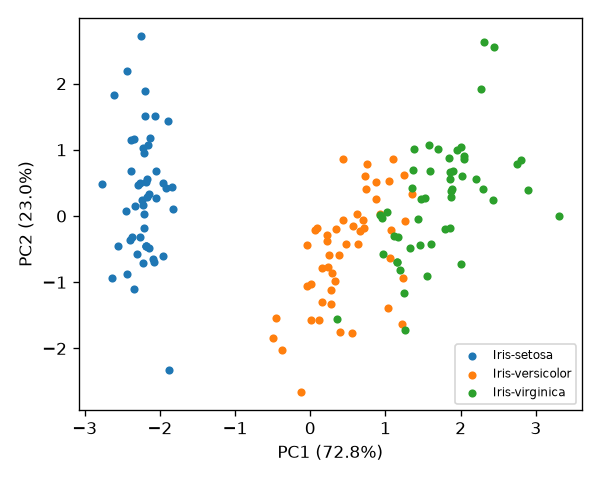
\includegraphics[height=4.2cm]{fig_pca.png}
\end{center}

\textbf{3. Distribuição das classes.} As variáveis de pétala separam melhor as classes.
A setosa não se sobrepõe às outras duas. Versicolor e virginica se sobrepõem pouco.
Na sépala, as três classes se sobrepõem bastante.

\textbf{4. PCA} (dados padronizados). PC1 explica 72,8\% da variância e PC2 explica 23,0\%.
Juntas, elas explicam 95,8\%. PC1 soma \texttt{sepal\_length}, \texttt{petal\_length} e \texttt{petal\_width}
(pesos 0,52, 0,58 e 0,57): ela mede o ``tamanho da flor''.
PC2 é quase só \texttt{sepal\_width} (peso 0,93).
No plano PC1$\times$PC2, a setosa fica isolada. Versicolor e virginica se tocam em uma região pequena.

\textbf{5. K-NN.} Divisão 80\% treino (120) e 20\% teste (30), com \texttt{train\_test\_split} (\texttt{random\_state=42}).
Distância euclidiana, variáveis padronizadas com média e desvio do treino.
\begin{center}\footnotesize
\begin{tabular}{lcc}
\toprule
Entrada & $k$ & Acurácia no teste \\
\midrule
4 variáveis & 1, 3, 5, 7, 9, 11, 15 & 1,000 (todos) \\
PC1 + PC2 & 1 / 5 / 11 & 0,867 / 0,933 / 0,900 \\
\bottomrule
\end{tabular}
\end{center}
Com as 4 variáveis, a matriz de confusão é diagonal: nenhum erro (10 setosa, 9 versicolor, 11 virginica).
Com PC1 e PC2, os erros ocorrem entre versicolor e virginica.

\textbf{Conclusões.}
\begin{itemize}
\item A setosa é linearmente separável das outras duas classes. Só versicolor e virginica podem ser confundidas.
\item O K-NN acerta 100\% no teste para todos os $k$ testados.
\item O teste tem só 30 amostras. Um erro muda a acurácia em 3,3 pontos. Por isso, 100\% não prova que o modelo é perfeito.
\item O PCA reduz de 4 para 2 dimensões e perde cerca de 4\% da variância. Essa perda custa de 7 a 13 pontos de acurácia.
\end{itemize}
\end{document}
